\chapter{Design}

In this section, the benchmark problem will be defined and mapped as DCOP, the framework design will be explained and the mapping of the algorithms on to the Signal/Collect framework will be described. Additionally, the design and considerations regarding the implemented monitoring platform are detailled.

\section{Meeting Scheduling Problem}

\subsection{Formal Definition as DCOP}

- General problem and definitions
- hard constraints Different, Same (sources for that)

\cite{Chapman2011}
chun, andy 2003
grubshtein
mes, martijn 2007


- timeslot utility design: first slot preference, preferences, soft constraints (free slots, 'blocked' slots)

Rajiv T. Maheswaran, Milind Tambe, Emma Bowring, Jonathan P. Pearce, and Pradeep Varakantham. Taking DCOP
to the real world: Efficient complete solutions for distributed multi-event scheduling.

DCOP Formulations for DiMES Now that we have captured our problem in the DiMES framework, we need an
approach to find an (optimal) solution.
A DCOP is defined as a tuple < A, X, D, R > [2] where A is a finite set of agents A = {A1, ..., Am}, X is a set
of variables X = {x1, ..., xN } distributed among the agents in A (each variable belongs to a unique agent), D is a set of
domains D = {D1, ..., DN } where a domain Di is the set of values that variable Xi can take. Finally R is a set of relations
R = r1...rp such that every relation defines a cost for the combinations of values from D, ri : Di1x..xDik R
The goal is to choose values for variables to optimize an objective function, the utility.
The convertion from a DiMES to a DCOP can be made in 3 different ways [6]:
TSAV (Time Slots As Variables): a variable Xn(t) is the n-th resources t-th time slot.
 The complexity of TSAV grows if the time range increases or the time quantization interval decreases.
EAV (Event As Variables): X
K represents the starting time of E
K, with domain t, ..., t
PEAV (Private Events As Variables): A modification of EAV to ensure privacy protection for agents information.
As in EAV each participant controls a private variable corresponding to the starting time of a meeting. But the
difference is that in this formulation agents dont share their internal valuation for the resources, thus maintaining
privacy. The experimental results in shows that EAV outperforms PEAV by one order of magnitude when using
passup in meeting scheduling. As in this project it is fundamental to preserve agents preferences as well as to have
the best variable control scheme we will consider only PEAV formulation.

Multi-agent meeting scheduling with preferences:
efficiency, privacy loss, and solution quality Franzin

problem density, etc

\subsection{Problem Generation}

- Decision: Available datasets are not usable because it was not possible to scale to high numbers. It was chosen to create problems randomly.
Frodo2

- brauche ein paar papers die das untermauern

- participations fixed
- 

Distributed Meeting Scheduling: CHAPTER 10

\section{Framework}

\subsection{Foundation}

It was decided to build a specific framework for benchmarking dynamic problems. The foundation of the framework is the signal/collect framework \cite{Stutz2010}\footnote{http://uzh.github.io/signal-collect}, which is built on top of Akka\footnote{http://akka.io} and written in Scala\footnote{http://www.scala-lang.org}. It is a graph processing engine with a programming model that features vertices and edges. The vertices have a state and send signals along the edges to other vertices, which can contain any datatype. The signal usually is their state or in context of their state. The vertices collect the signals and perform a compution on the collected data, before adjusting their state according to the calculations and sending out the newly generated signal.  This model allows to reduce complex algorithms to a few lines of code and is applicable for many problems.\newline\newline
The reason for choosing this framework in this thesis is the structural fit to distributed constraint optimization problems and the possiblity to add and remove vertices during runtime. This allows for dynamically changing problem computations. Further, the capability of running problems asynchronously or with synchronous signal steps and the possibility to distribute the system on multiple machines add to the advantages.

\subsection{Parameters \& Modes}
This framework was designed with the benchmarks in mind.  It should be possible to pass the general run parameters like which algorithm to use, which Signal/Collect run mode (synchronous/asynchronous) to use, normal run mode or dynamic variations (changeConstraints, changeVariable, changeDomain) with specific parameters. For testing, two test modes were implemented: SingleTest and MultiTest. Single Test is for single runs obviously and MultiTest allows to specifiy how many runs each specification should be doing to create a median of those runs, how much the agents respectively the meetings should increase after a specification has been processed and where to stop. By this, it is possible to explore an area of specifications. Finally, it should be possible to define different problems. For this thesis, the parameters for problem density (blocked timeslots percentage), timeslots, meetings and agents were defined.

\subsection{Functionality \& Structure}

The considerations for the structure were that I needs to be hierarchical to allow different constraint optimization problems to be run on the framework. So, the hierachy goes from a Base to a Dynamic to a Problem level. It should include ProblemFactories and Problems, GraphFactories and Graphs, as well as Vertices.\newline\newline

- Problem Factory: Problem -> MeetingSchedulingProblem class diagram

- Graph Factory: Graph -> DPOP Graph, MGM Graph, MaxSum Graph explanation 
- Graph

- BasicVertex -> DynamicVertex -> MeetingSchedulingVertex -> DPOP, MGM, MaxSum Vertex class diagram!!!

\subsection{Dynamics Controller}

how does it work, what can it do

- Registration of vertices
- change constraints
- change variables
- change domain

- Initial design consideration was to make it part of the graph as signal collect allows mixup of different types. Created weird problems because I need to pause the vertex for interval changes. not part of the graph but connected to vertices -> because it was a problem with convergence and there was a problem with thread sleep in akka

\section{Mapping of DPOP}

based on: A Scalable Method for Multiagent Constraint Optimization
    
    - Why DPOP
    DPOP is a primary example for a complete algorithm
   
    \begin{algorithm}
\caption{My algorithm}\label{euclid}
\begin{algorithmic}[1]
\Procedure{MyProcedure}{}
\State $\textit{stringlen} \gets \text{length of }\textit{string}$
\State $i \gets \textit{patlen}$
\BState \emph{top}:
\If {$i > \textit{stringlen}$} \Return false
\EndIf
\State $j \gets \textit{patlen}$
\BState \emph{loop}:
\If {$\textit{string}(i) = \textit{path}(j)$}
\State $j \gets j-1$.
\State $i \gets i-1$.
\State \textbf{goto} \emph{loop}.
\State \textbf{close};
\EndIf
\State $i \gets i+\max(\textit{delta}_1(\textit{string}(i)),\textit{delta}_2(j))$.
\State \textbf{goto} \emph{top}.
\EndProcedure
\end{algorithmic}
\end{algorithm}

\subsection{Graph Structure}
\subsection{Vertices}

\section{Mapping of MGM}

     - Why MGM
     Good example for Best-Response algorithm and DSA-B has already been implemented

    \begin{algorithm}
\caption{My algorithm}\label{euclid}
\begin{algorithmic}[2]
\Procedure{MyProcedure}{}
\State $\textit{stringlen} \gets \text{length of }\textit{string}$
\State $i \gets \textit{patlen}$
\BState \emph{top}:
\If {$i > \textit{stringlen}$} \Return false
\EndIf
\State $j \gets \textit{patlen}$
\BState \emph{loop}:
\If {$\textit{string}(i) = \textit{path}(j)$}
\State $j \gets j-1$.
\State $i \gets i-1$.
\State \textbf{goto} \emph{loop}.
\State \textbf{close};
\EndIf
\State $i \gets i+\max(\textit{delta}_1(\textit{string}(i)),\textit{delta}_2(j))$.
\State \textbf{goto} \emph{top}.
\EndProcedure
\end{algorithmic}
\end{algorithm}

\subsection{Graph Structure}
\subsection{Vertices}

\section{Mapping of MaxSum}

\cite{Yedidsion}
Farinelli2008
zivan2012
    
    - Why MaxSum
    MaxSum is the new kid on the block.

    \begin{algorithm}
\caption{My algorithm}\label{euclid}
\begin{algorithmic}[3]
\Procedure{MyProcedure}{}
\State $\textit{stringlen} \gets \text{length of }\textit{string}$
\State $i \gets \textit{patlen}$
\BState \emph{top}:
\If {$i > \textit{stringlen}$} \Return false
\EndIf
\State $j \gets \textit{patlen}$
\BState \emph{loop}:
\If {$\textit{string}(i) = \textit{path}(j)$}
\State $j \gets j-1$.
\State $i \gets i-1$.
\State \textbf{goto} \emph{loop}.
\State \textbf{close};
\EndIf
\State $i \gets i+\max(\textit{delta}_1(\textit{string}(i)),\textit{delta}_2(j))$.
\State \textbf{goto} \emph{top}.
\EndProcedure
\end{algorithmic}
\end{algorithm}

\subsection{Graph Structure}
\subsection{Vertices}

\section{Monitoring Platform}

It was decided to find a more sophisticated method to monitor the utility, quality, conflicts and stats of the calculations than to write to a logfile. Partially because File IO can possibiliy be limited in the number of open files and processing results to fit the log file format during calculations can affect the performance of the algorithm one tries to benchmark. Mainly because processing log files was to tedious and visibility was not given to the calculations.

Sending the results with non-blockin http requests to a restful server was considered to be an alternative and the Play Framework\footnote{https://www.playframework.com} has been chosen because it is highly scalable, is able to handle thousands of simultanous connections, lightweight, non-blocking and allows to process results on-the-fly with code in Java or Scala. It was also chosen because Akka is tightly integrated and the actors concept are an integral part of the framework. It further allows to preview the calculation of the graph in realtime with websockets, which can be helpful during the implementation of algorithms.

By using an actor based approach it is possible to contain run specific data in a closed entity and store when limits are reached. Through the chosen architecture one can run multiple tests in parallel without problems. The server is of course also limited by it's ressources.

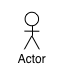
\includegraphics{graphics/monitoring}


